\section*{Projects}
\begin{frame}{Sim Racing Series}
    \begin{columns}
        \column{0.6\textwidth}
        The Sim Racing Series is a yearly
        sim racing challenge using Assetto Corsa.
        \begin{itemize}
            \item 6 rounds, beginning in November
            \item Practice server opens before race
            \item Tune the setup of the car
            \item Set the fastest laptime possible
            \item Finals held at Williams in July
            \item \href{https://www.imeche.org/events/formula-student/team-information/fs-sim-racing}{\textit{More info on the IMechE website}}
        \end{itemize}
        Charlie Spence will be leading it this year.
        Intro meeting at 6pm on Tuesday 21st October on Discord.
        \column{0.4\textwidth}
        \begin{figure}
            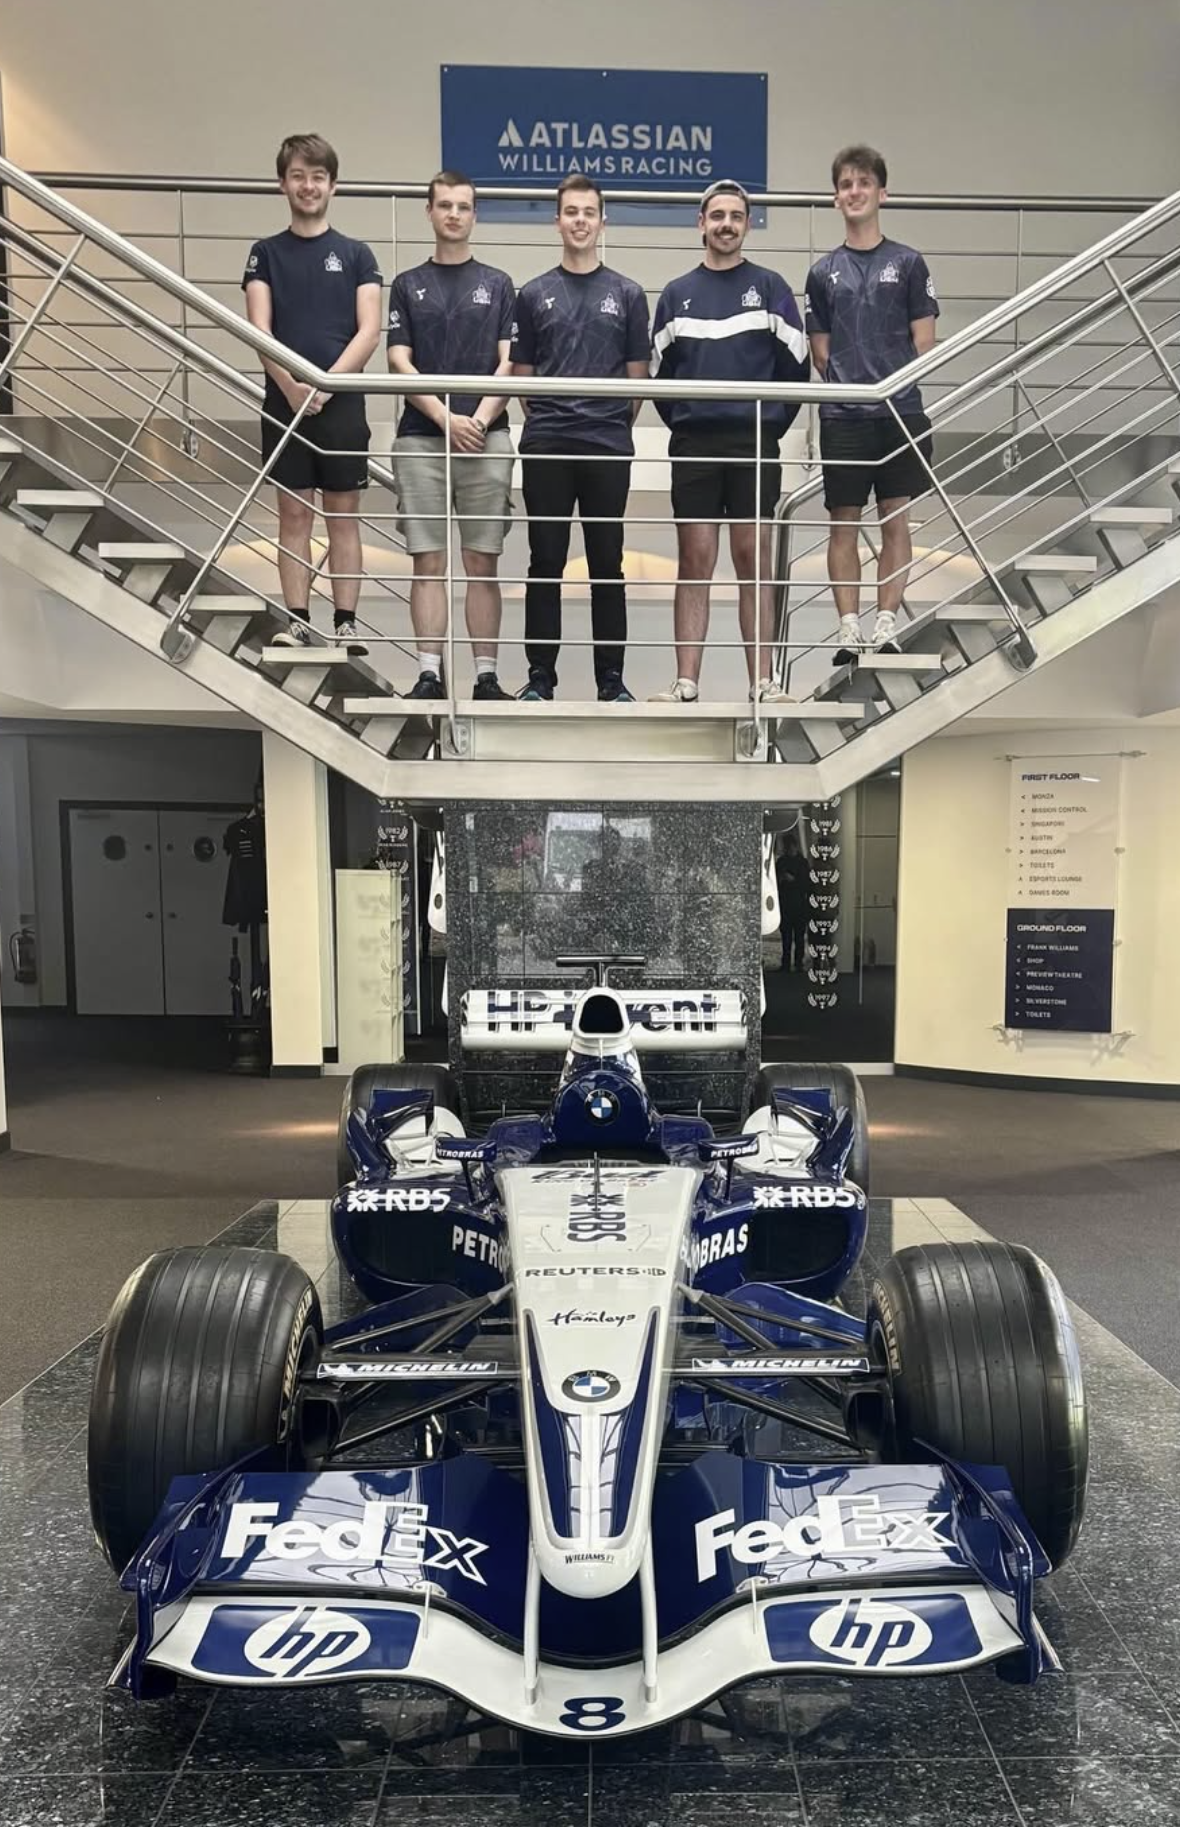
\includegraphics[width=\textwidth]{res/Williams Sim Racing.png}
        \end{figure}
    \end{columns}
\end{frame}

\begin{frame}{Driver Development}
    8 drivers have been selected for this season.
    We will be running driver development sessions with them. \\
    \vspace{2ex}
    I'd like to start training people as race engineers:
    \begin{itemize}
        \item Monitor our drivers' performance
        \item Analyse data using Race Studio
        \item Identify issues with the vehicle or driving style
        \item Gather feedback on vehicle handling
    \end{itemize}
    I'll hopefully organise some teaching sessions
    on using software and analysing data.
\end{frame}

\begin{frame}{Mock Engineering Challenge}
    The Engineering Challenge is a series of scenarios
    where you must act as a race engineer
    to tune  the setup and performance of a car. \\
    \vspace{2ex}
    To prepare for the first challenge (beginning in November),
    we will run a mock engineering challenge.
    You will be split into teams
    (ideally a sim driver + a race engineer). \\
    \vspace{2ex}
    I will release the details of the challenge next week.
    You will have 3 weeks to look at the problem,
    run some test laps with different setups,
    and create a short report.
\end{frame}

\begin{frame}{Coding Projects}
    Some coding projects which have been requested by the team:
    \begin{itemize}
        \item \textbf{Mass distribution calculator:}
        how does changing the position of a part
        affect the position of the centre of mass?
        \item \textbf{Suspension compliance model:}
        how much do the suspension links deform under load?
        \item \textbf{Competitor analysis:}
        use the competitor database from the new member project
        to make some graphs of parameters vs performance
        \item \textbf{Setup sheet:}
        write some code to generate a vehicle setup sheet
        or read values from it
    \end{itemize}
    You can choose which language you use
    (MATLAB or Python recommended).
    I'll review the code with you,
    then it can be used by the team.
\end{frame}